%*************************************************************************
%* Copyright © 2012-2014 Vincent Prat & Simon Nicolas
%*
%* This document is free; you can redistribute it and/or modify
%* it under the terms of the GNU General Public License as published by
%* the Free Software Foundation; either version 3 of the License, or
%* (at your option) any later version.
%*
%* This document is distributed in the hope that it will be useful,
%* but WITHOUT ANY WARRANTY; without even the implied warranty of
%* MERCHANTABILITY or FITNESS FOR A PARTICULAR PURPOSE. See the
%* GNU General Public License for more details.
%*
%* You should have received a copy of the GNU General Public License along
%* with this document; if not, write to the Free Software Foundation, Inc.,
%* 51 Franklin Street, Fifth Floor, Boston, MA 02110-1301 USA.
%*************************************************************************

\documentclass[a4paper,12pt]{article}

\usepackage[frenchb]{babel}
\usepackage[utf8]{inputenc}
\usepackage{graphicx}
\usepackage{hyperref}
\usepackage{xspace}

\graphicspath{{images/}}

\newcommand*{\GMA}{GM-Assistant\xspace}
\newcommand*{\interfaceitem}[1]{\texttt{#1}}
\newcommand*{\guillemets}[1]{\og #1\fg{}\xspace}
\newcommand*{\versionnumber}{1.2\xspace}

\title{\GMA \versionnumber, guide de l'utilisateur}
\author{Simon Nicolas \and Vincent Prat}

\begin{document}

\maketitle

\tableofcontents

\section{Introduction}

Une partie de jeu de rôle est une alchimie riche et complexe.
Les joueurs doivent être impliqués et investis et le maître de jeu (ou MJ) doit parfaitement maîtriser le système de règle, le scénario, se rappeler des évènements précédents, anticiper les évènements à venir, et improviser le présent en fonction des actions et choix des joueurs.
Si en pleine partie le MJ doit chercher des détails sur un PNJ (personnage non joueur, c'est-à-dire non incarné par un joueurs), une précision sur un point de règle, des musiques d'ambiance ou des bruitages sur l'ordinateur, des images dans son classeur, ou autre, alors la partie ralentit, l'émulsion retombe, et les joueurs se dispersent.
Ne niez pas, un rôliste se disperse vite.

La solution est \GMA, pour \emph{Game Master Assistant} (en français, assistant au MJ).
Son objectif est de simplifier la vie du MJ en mettant à sa disposition les informations et outils dont il peut avoir besoin pendant la partie.
\GMA propose donc une interface où le MJ va pouvoir rassembler et ordonner toutes les informations, notes et fichiers (musiques, bruitages, images) qu'il estime utiles.

Cette documentation a pour but d'aider l'utilisateur (c'est-à-dire vous) à se familiariser avec le logiciel.
Pour cela, elle est divisée en deux grandes parties~: tout d'abord une présentation générale de l'interface du logiciel et de ses fonctionnalités (section~\ref{sec:pres}), puis dans un second temps un exemple d'utilisation de \GMA pour construire une fiche de scénario (section~\ref{sec:exem}).

\section{Présentation générale}
\label{sec:pres}

La fenêtre principale du logiciel comporte d'une part une barre de menus, qui sera développée dans la section~\ref{menu} et d'autre part 6 sous-parties que nous appellerons modules et qui seront présentés dans la section~\ref{sec:modules}.
Le logiciel propose également un certain nombre d'outils annexes qui feront l'objet de la section~\ref{sec:outils}.

\subsection{Présentation des menus}
\label{menu}

La barre de menus de \GMA est similaire à celle que l'on trouve dans la plupart des logiciels.
Nous allons maintenant détailler un par un les menus principaux, qui sont \interfaceitem{Jeu} (section~\ref{sec:jeu}), \interfaceitem{Édition} (section~\ref{sec:edition}), \interfaceitem{Affichage} (section~\ref{sec:affich}), \interfaceitem{Outils} (section~\ref{sec:menu_outils}) et \interfaceitem{Aide} (section~\ref{sec:aide}).

\subsubsection{Jeu}
\label{sec:jeu}

Ce menu comprend tous les outils de gestion et de sauvegarde des fiches de scénarios créées avec \GMA.
En voici la liste~:
\begin{description}
    \item[\interfaceitem{Nouveau}~:]{crée une nouvelle fiche de scénario vide}
    \item[\interfaceitem{Recharger}~:]{restaure la fiche de scénario courante telle qu'elle était lors de la dernière sauvegarde}
    \item[\interfaceitem{Charger}~:]{charge une fiche de scénario stockée sur l'ordinateur}
    \item[\interfaceitem{Récents}~:]{propose la liste des fiches de scénario récemment ouvertes}
    \item[\interfaceitem{Enregistrer}~:]{sauvegarde la fiche de scénario en cours d'édition}
    \item[\interfaceitem{Enregistrer sous}~:]{sauvegarde la fiche de scénario en cours d'édition dans un nouveau fichier}
    \item[\interfaceitem{Métadonnées}~:]{affiche une fenêtre permettant de noter le titre du scénario, son auteur, la date de création, une description sommaire, le jeu de rôle, la liste des joueurs et la date de jeu.
            L'idée est rassembler des informations qui ne servent pas en partie mais qui permettent de se souvenir de \guillemets{Qui~? Quand~? Comment~?}.}
    \item[\interfaceitem{Quitter}~:]{ferme la fiche de scénario en cours et quitte le logiciel}
\end{description}
\paragraph{Le fichier de sauvegarde}
Le fichier de sauvegarde \texttt{.gms} créé est un fichier complet qui comprend toutes les informations qui sont dans la fiche de scénario et les fichiers annexes que vous y avez ajouté (musique, bruitages, images), lui permettant d'être déplacé d'un ordinateur à un autre sans risque de perte (un son manquant ou une image absente par exemple).

\subsubsection{Édition}
\label{sec:edition}

Ce menu a pour but d'aider l'utilisateur lors de l'élaboration de la fiche de scénario.
Pour l'instant, il se compose uniquement de deux actions~:
\begin{description}
    \item[\interfaceitem{Annuler}~:]{annule la dernière modification apportée}
    \item[\interfaceitem{Refaire}~:]{rétablit la dernière modification apportée après son annulation}
\end{description}

\subsubsection{Affichage}
\label{sec:affich}

Ce menu permet de choisir parmi différentes options d'affichage.
Il se compose de deux sous-menus~:
\begin{description}
    \item[\interfaceitem{Interface}~:]{ouvre la liste des arrangements de modules disponibles (voir la section~\ref{sec:modules} pour la description de chacun des modules).
        Chaque interface propose un appariement différent de modules~:
        \begin{description}
            \item[\interfaceitem{Complète}~:]{est composée des 6 modules}
            \item[\interfaceitem{Simple}~:]{est composée des modules \interfaceitem{Intrigue}, \interfaceitem{Musique} et \interfaceitem{Bruitage}}
            \item[\interfaceitem{Musique}~:]{est composée des modules \interfaceitem{Musique} et \interfaceitem{Bruitage}}
            \item[\interfaceitem{Conception}~:]{est composée des modules \interfaceitem{Intrigue}, \interfaceitem{Personnages} et \interfaceitem{Notes}}
            \item[\interfaceitem{Sans son}~:]{est composée des modules \interfaceitem{Intrigue}, \interfaceitem{Historique}, \interfaceitem{Personnages} et \interfaceitem{Notes}}
        \end{description}
    }
    \item[\interfaceitem{Langue}~:]{ouvre la liste des langues disponibles pour l'interface graphique du logiciel.
        Actuellement, seuls l'anglais et le français sont supportés.}
\end{description}

\subsubsection{Outils}
\label{sec:menu_outils}

Ce menu rassemble les différents outils annexes proposés par \GMA.
Le fonctionnement de ces outils sera abordé en détail dans la section~\ref{sec:outils}.
Dans la présente version du logiciel, le menu comprend~:
\begin{description}
    \item[\interfaceitem{Simulateur de dés}~:]{permet de simuler le lancer d'un certain nombre de dés d'un certain type}
    \item[\interfaceitem{Gestionnaire de combat}~:]{outil permettant de structurer le déroulement des combat}
\end{description}

\subsubsection{Aide}
\label{sec:aide}

Ce menu donne accès aux informations générales sur le logiciel et sa licence.

\subsection{Présentation des modules}
\label{sec:modules}

Comme évoqué précédemment, la fenêtre principale du logiciel est découpée en six blocs indépendants et dédiés chacun à une fonctionnalité, appelés modules.
Plusieurs de ces modules se présentent sous forme d'un arbre \guillemets{dépliable} permettant d'organiser des informations.
Les possibilités offertes par ces arbres et les items qui les composent seront développées dans la section~\ref{item}.
Voici la liste des modules présents dans cette version~:
\begin{description}
    \item[\interfaceitem{Intrigue}~:]{arbre qui permet d'afficher de manière ordonnée les différents évènements important du scénario (voir la section~\ref{sec:intrigue} pour plus de détail)}
    \item[\interfaceitem{Historique}~:]{encore un arbre, qui a cette fois vocation à rappeler les évènements les plus marquants des scénarios précédents ou du passé des personnages (voir section~\ref{sec:historique})}
    \item[\interfaceitem{Notes}~:]{éditeur de texte simpliste qui permet de prendre des notes avant ou pendant la partie (voir section~\ref{sec:notes})}
    \item[\interfaceitem{Personnages}~:]{tableau permettant d'afficher les protagonistes (PJ ou PNJ) avec leurs caractéristiques importantes (voir section~\ref{sec:perso})}
    \item[\interfaceitem{Musique}~:]{lecteur de musique simple pensé pour jouer des musiques d'ambiance (voir section~\ref{sec:musique})}
    \item[\interfaceitem{Bruitages}~:]{lecteur de musique encore plus simple pensé pour jouer des bruitages courts (voir section~\ref{sec:bruitages})}
\end{description}
Tout ces modules sont rassemblés dans l'interface par défaut du logiciel, comme on peut le voir sur la figure~\ref{fig:interface}, mais peuvent également être réorganisés grâce au sous-menu \interfaceitem{Interface} du menu \interfaceitem{Affichage} décrit précédemment dans la section~\ref{sec:affich}.
\begin{figure}[h]
    \includegraphics[width=0.9\textwidth]{screen_scenar_exemple}
    \caption{Fenêtre principale du logiciel avec une partie en cours}
    \label{fig:interface}
\end{figure}

\subsubsection{La notion d'item}
\label{item}

Les items sont à la base du fonctionnement de \GMA, il est donc approprié d'en expliquer le fonctionnement avant de détailler les modules.
Par définition, un item désigne un élément minimal d'un ensemble.
Dans notre cas, un item est une ligne, une entrée dans un des modules sous forme d'arbre du logiciel, qui sert à contenir une information textuelle, un son (musique ou bruitage), une image, etc.
Les modules qui utilisent les items sont \interfaceitem{Intrigue}, \interfaceitem{Historique}, \interfaceitem{Musique} et \interfaceitem{Bruitage}.

Chaque item se présente comme une ligne de texte dans un certain état et d'un certain type.
L'état d'un item permet de prendre note rapidement du succès ou de l'échec de certains points clefs du scénario, et d'en avoir une vision rapide.
Les quatre états disponibles sont \interfaceitem{Aucun}, \interfaceitem{En cours}, \interfaceitem{Échoué} et \interfaceitem{Réussi}.
Le type d'un item détermine sa fonction.
Dans cette version du logiciel, un item peut être \interfaceitem{Basique} (uniquement du texte), \interfaceitem{Audio} (musiques et bruitages) ou \interfaceitem{Image}.

Nous allons maintenant décrire le fonctionnement des arbres.
Lorsque vous cliquez avec le bouton droit de la souris sur un item apparaît le menu de gestion d'item.
Ce menu contient les quatre états possible d'un item puis les trois actions \interfaceitem{Ajouter}, \interfaceitem{Supprimer} et \interfaceitem{Éditer}.
Si l'item est de type \interfaceitem{Audio} ou \interfaceitem{Image}, une action supplémentaire est présente pour jouer le fichier audio ou afficher l'image.
Veuillez noter que pour les fichiers audio, cette action n'apparaît que dans les modules \interfaceitem{Musique} et \interfaceitem{Bruitages}.

L'action \interfaceitem{Ajouter} nous permet d'accéder à la fenêtre de création d'item (figure~\ref{fig:ajout}).
\begin{figure}[h]
    \includegraphics[width=0.5\textwidth]{screen_add_item}
    \caption{Fenêtre de création d'item}
    \label{fig:ajout}
\end{figure}
Notez qu'il est également possible d'accéder à cette fenêtre en cliquant avec le bouton droit de la souris dans la partie vide du module ou en appuyant sur la touche \interfaceitem{Inser} de votre clavier.
Voici comment s'organise cette fenêtre~:
\begin{itemize}
    \item le cadre \interfaceitem{Contenu} reçoit la description de l'évènement~;
    \item le cadre \interfaceitem{État} permet de fixer l'état de l'item~;
    \item le cadre \interfaceitem{Type} permet de choisir le type de l'item et pour les items de type \interfaceitem{Audio} et \interfaceitem{Image} de sélectionner le fichier correspondant~;
    \item Le bouton \interfaceitem{Ajouter} ajoute l'item à la suite et au même niveau que l'item sur lequel on a cliqué avant d'ouvrir la fenêtre (si aucun item n'était sélectionné, ajoute simplement l'item à la suite au niveau le plus bas)~;
    \item Le bouton \interfaceitem{Enfant} ajoute l'item à la suite et sous l'item sur lequel on a cliqué précédemment, imbriqué dedans~;
    \item Le bouton \interfaceitem{Annuler} annule la création d'item en cours.
\end{itemize}
Il est important de bien saisir la différence entre les deux boutons \interfaceitem{Ajouter} et \interfaceitem{Enfant}, car c'est grâce à eux que vous organiserez les étapes de votre scénario.
Une fois créés, les items sont également déplaçables au sein d'un même module par \guillemets{glisser-déposer}.

L'action \interfaceitem{Éditer} ouvre une fenêtre similaire à celle de création d'item, la seule différence importante étant qu'il n'y a plus \interfaceitem{Ajouter} et \interfaceitem{Enfant}, mais uniquement un bouton \interfaceitem{Valider} permettant de valider l'édition.
Si vous voulez uniquement modifier le texte d'un item, il vous suffit d'appuyer sur la touche \interfaceitem{F2} de votre clavier (la combinaison \interfaceitem{Ctrl+F2} ouvre quant à elle la fenêtre d'édition).

\subsubsection{Intrigue}
\label{sec:intrigue}

L'arbre d'intrigue est dans la majorité des cas le cœur de \GMA.
En effet, vous pouvez entrer dedans le plan détaillé et ordonné du scénario, de manière à ne jamais être perdu entre deux scènes ni oublier un élément.
\\
Voir figure(\ref{arbre_scenar}) pour un aperçu de ce qu'il est possible de faire
\begin{figure}[h]
    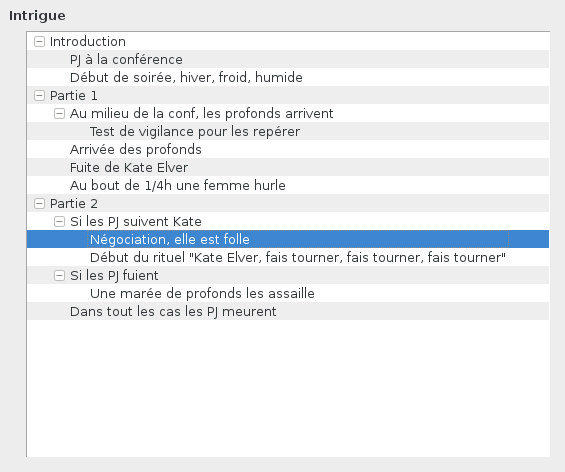
\includegraphics[width=0.6\textwidth]{scenario_type}
    \caption{Plan schématique d'un scénario}
    \label{arbre_scenar}
\end{figure}
Donc comment faire ?
\\
chaque ligne que vous voyez est un \emph{item}, il suffit de suivre la technique de création d'item pour ordonner son scénario.

\subsubsection{Historique}
\label{sec:historique}

L'arbre d'historique sert à se préparer une liste des évènements importants ayant marqués les séances précédentes, commme la rencontre des personnages, une promesse faite par un PJ à un PNJ (ou l'inverse), etc.
Il se comporte et s'utilise (d'un point de vue technique) exactement de la même manière que l'arbre de Scénario.


\subsubsection{Notes}
\label{sec:notes}

Le module de prise de note est un éditeur de texte ultra simpliste qui permet de noter à la volée toute information qui est utile à garder (exemple : "Sylvain a insulté le directeur du museum"). Pour entrer du texte dedans il suffit de cliquer gauche quelque part dans le cadre texte et d'écrire.
\\
%\emph{Nota Bene :} ce module sera rapidement accessible lorsque la fonctionnalité de \emph{suivi de campagne} sera implémentée.

\subsubsection{Personnages}
\label{sec:perso}

Le module \interfaceitem{Personnages} est pensé pour accueillir la liste des protagonistes ainsi que les caractéristiques numériques dont vous pouvez avoir besoin rapidement. Que ce soit des PJ pour lesquels on a besoin des scores de Perception, vigilance, esquive passive, des points de vie etc. ou directement des caractéristiques complètes des PNJ.
\\
Liste des actions possibles :
\begin{itemize}
    \item Clic droit dans la partie vide puis \interfaceitem{Propriété}~: ajoute une propriété sur le bandeau horizontale;
    \item Clic droit dans la partie vide puis \interfaceitem{Personnage}~: ajoute un personnage sur le bandeau vertical.
\end{itemize}
Ensuite une fois qu'on a créé au moins un personnage et une compétence alors la case est éditable. Il faut maintenant cliquer gauche pour éditer la case voulue et y entrer la valeur.
\\\emph{Nota bene :} il est possible d'entrer du texte, des nombres, mais aussi d'autre caractères comme le "\%"

\subsubsection{Musique}
\label{sec:musique}

Le module de musique d'ambiance est un lecteur de musique basique (loin des Winamp et autres VirtualDJ) qui permet de jouer une musique (au format MP3).
\\
Liste des actions possibles :
\begin{itemize}
    \item Actions des items (\emph{cf.} section~\ref{item})
    \item Clic gauche \interfaceitem{Lecture/Pause}~: s'il n'y a pas de lecture en cours c'est le bouton \interfaceitem{Lecture} qui est affiché. CLiquer dessus joue le son sélectionné; lorsqu'une lecture est en cours le bouton change en bouton \interfaceitem{Pause} qui est affiché. Cliquer dessus met la lecture en pause.
    \item Clic gauche sur la case blanche \interfaceitem{Boucle}~: active le mode répétition donc joue en boucle la musique de cours de lecture;
    \item Clic gauche déplacer sur la barre d'avancement~: permet de se déplacer dans le son.
\end{itemize}
\emph{Nota Bene :} il est impossible de jouer 2 musiques en même temps.

\subsubsection{Bruitages}
\label{sec:bruitages}

Le module de bruitage est pensé pour accueillir une liste de son très court (au format MP3) comme un coup de feu, un hurlement, une porte qui claque, etc.
\\
Liste des actions possibles :
\begin{itemize}
    \item Actions des items cf (\ref{item})
    \item Double clic gauche sur un item:joue le bruitage
\end{itemize}

\emph{Nota Bene :} Il est tout fait possible de jouer un bruitage alors qu'une musique est en cours de lecture.

\subsection{Présentation des outils}
\label{sec:outils}

\subsubsection{Le simulateur de dé}
Le simulateur de dé est un outil permettant de s'affranchir du lancé de dé en reproduisant directement dans le logiciel l'aléatoire des dés.
Cet outil se trouve dans le menu \interfaceitem{Outils}
Vous obtenez la fenêtre (\ref{simulateur_de}).
\begin{figure}[h]
    \includegraphics[width=0.6\textwidth]{simulateur_de_de}
    \caption{Simulateur de dé}
    \label{simulateur_de}
\end{figure}

Elle comprend les éléments suivant :
\begin{itemize}
  \item  \emph{type de dés} permet de choisir le nombre de faces qu'auront les dés.
  \item \emph{nombre} permet de choisir combien de dés, jusqu'à concurrence de 10.
\end{itemize}
Ensuite on clique sur "Lancer" et le résultat s'affiche dans le cadre blanc.

\subsubsection{Le gestionnaire de combat}
Quand on lance le gestionnaire de combat on arrive sur la fenêtre (\ref{gestion_combat_choix}) de selection de personnage.
\begin{figure}[h]
    \includegraphics[width=1\textwidth]{gestionnaire_combat_1}
    \caption{Gestionnaire de combat : préparation}
    \label{gestion_combat_choix}
\end{figure}
La liste des personnages est générée automatiquement à partir des protagonistes entrés dans le module \interfaceitem{Personnages}.
On choisi chaque participant au combat en le sélectionnant dans la colonne de gauche et en l'ajoutant à la colonne de droite en cliquant sur \interfaceitem{Ajouter}.
On ajoute les différents acteurs, dans l’ordre de leurs actions, si certains
agissent plusieurs fois par tour il suffit de les ajouter plusieurs fois. Les flèches \interfaceitem{Haut} et \interfaceitem{Bas} à droite permettent de réorganiser l’ordre des actions.
Une fois la préparation terminée on valide en cliquant \interfaceitem{Ok}.
Apparait maintenant le gestionnaire de combat lui-même (\ref{gestion_combat_fight}
\begin{figure}[h]
    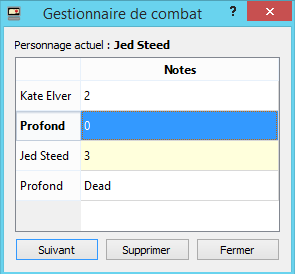
\includegraphics[width=0.4\textwidth]{gestion_combat_fight}
    \caption{Gestionnaire de combat : action}
    \label{gestion_combat_fight}
\end{figure}
Ensuite à chaque round de combat on clique sur \interfaceitem{Suivant}, la ligne \interfaceitem{Personnage actuel :} indique quel personnage agit. En cas de blessure ou commentaire spécifique il est possible d'ajouter du texte dans la colonne \interfaceitem{Notes} en double-cliquant dessus.
En cas de sortie du combat pour un personnage (fuite, mort, etc.) il suffit de cliquer sur \interfaceitem{Supprimer}, pour retirer ce personnage du gestionnaire.

Une fois le combat terminé il suffit de cliquer sur \interfaceitem{Fermer}

\section{Exemple : Construire la fiche d'un scénario}
\label{sec:exem}

Maintenant que nous avons fait le tour des fonctionnalités du logiciel, construisons ensemble la "fiche scénario" du scénario exceptionnel (et exclusif) : \emph{La nuit tous les profonds sont gris}.

\subsection{Présentation du scénario}
\label{exemple_scenario}
Le Scénario
\begin{itemize}
    \item \emph{Titre du scénario :} La nuit tous les profonds sont gris
    \item \emph{Jeux de rôle :} L'appel de Cthulhu
    \item \emph{Année :} 1920
    \item \emph{Lieux :} Toulouse
    \item \emph{Nombre de joueurs : } 4
\end{itemize}

\emph{Scénario :}\\ 
Les PJ sont au vernissage d'une exposition au laboratoire de pharmacologie de la faculté de médecine située allée Jules Guesde à Toulouse. Cependant ce laboratoire hébèrge  un étrange squelette retrouvé récemment au fond de l'eau. Au cours de la soirée des profonds sortent de la garonne pour récupérer le-dit squelette, qui est en fait la dépouille d'un de leur chaman.
\\
En même temps une des convives, Kate Elver, est une sorciere qui veut utiliser ce squelette pour en extraire de la puissance. Elle profitera de la cohue des convives lors de l'assaut des profonds pour aller dans le laboratoire, et commencer son rituel. La suite dépend des PJ. Si le rituel va au bout une onde de choc jette tout le monde à terre et les profonds fou de rage d'avoir perdu leur chaman définitivement assassinent tout le monde, sinon ils repartent "tranquillement" avec leur chaman (squelette).

\subsection{Les Métadonnées}
La première étape est de remplir les métadonnées. À partir des informations du scénario nous renseignons donc la fenêtre dédiée: (figure~\ref{metadata}).
\begin{figure}[h!]
    \includegraphics[width=0.6\textwidth]{metadata}
    \caption{fenêtre métadonnées}
    \label{metadata}
\end{figure}
Puis validons en cliquant gauche \interfaceitem{OK}.

\subsection{L'Intrigue}
Rentrons maintenant le plan du scénarion en ajoutant dans le module \interfaceitem{Intrigue} les différentes étapes clef du scénario.
\\
Commençons par cliquer gauche dans le cadre blanc. La fenêtre (\ref{intrigue_scenario}) apparait 
\begin{figure}[h!]
    \includegraphics[width=0.5\textwidth]{intrigue_intro}
    \caption{fenêtre d'ajout d'item}
    \label{intrigue_scenario}
\end{figure}
Nous allons écrire \interfaceitem{Introduction} puis détailler l'intro dans les item "fils".
Clic droit sur \interfaceitem{Introduction}, \interfaceitem{Ajouter}, nous arrivons sur la fenêtre d'ajout d'item, ce coup-ci on va l'ajouter en "enfant", pour qu'il apparaisse imbriqué sous \interfaceitem{Introduction} (voir figure~\ref{item_enfant}).
\begin{figure}[h!]
    \includegraphics[width=0.5\textwidth]{item_enfant}
    \label{item_enfant}
\end{figure}
Et on valide en cliquant gauche sur \interfaceitem{Enfant}.
On peut utiliser cette partie d'introduction pour se rappeler des différents élément d'ambiance à présenter aux joueurs.

Ensuite on ajoute la première partie du scénario. Clic droit dans la partie blanche, dans \interfaceitem{Contenu} on écrit \interfaceitem{Partie 1} et on valide par \interfaceitem{Ajouter} pour qu'il apparaisse à la suite de \interfaceitem{Introduction} et au même niveau.
On procède de la même manière pour les différentes étapes du scénario :
\begin{itemize}
    \item Introduction
    \begin{itemize}
        \item début de soirée, hivers, froid, humide
        \item PJ à la conférence
    \end{itemize}
    \item Partie 1
    \begin{itemize}
        \item Au milieu de la conf les profonds arrivent
        \begin{itemize}
            \item Test de "vigilance" pour les repérer
        \end{itemize}
        \item Arrivée des profonds
        \item Fuite de Kate Elver
        \item au bout de 1/4h une femme hurle
    \end{itemize}
    \item Partie 2
    \begin{itemize}
        \item Si les PJ suivent Kate
        \begin{itemize}
            \item Négociation, elle est folle
            \item début du rituel "Kate Elver, fais tourner x3"
        \end{itemize}
        \item Si les PJ fuient
        \begin{itemize}
            \item une marée de profonds les assaille
        \end{itemize}
    \end{itemize}
    \item Dans tout les cas les PJ meurent
\end{itemize}
voir le résultat sur la figure (\ref{intrigue_full}).  
\begin{figure}[h!]
    \includegraphics[width=0.8\textwidth]{intrigue_full}
    \caption{le scénario est prêt}
    \label{intrigue_full}
\end{figure}    
L'intrigue est prête mais pas notre scénario.

\subsection{Personnages}
Rentrons maintenant les différents protagonistes PNJ:
\begin{itemize}
    \item Kate Elver, la sorcière
    \item les guerriers profonds
    \item le shaman profond
\end{itemize}
et les PJ
\begin{itemize}
    \item Jed Steed, joué par Nathan
    \item Caleb de la muerta, joué par Yan
    \item Connara l'den, joué par Nico
\end{itemize}
Pour ajouter ces protagonistes commençons par cliquer droit dans la partie vide du module \interfaceitem{Personnages}, puis \interfaceitem{Personnage} et \interfaceitem{Ajouter} (figure~\ref{ajout_perso}).
\begin{figure}[h!]
    \includegraphics[width=0.4\textwidth]{ajout_perso}
    \caption{ajoutons Kate Elver}
    \label{ajout_perso}
\end{figure}
De la même manière nous allons ajouter tous les protagoniste, en mettant dans la seconde ligne une description sommaire (un ou deux mots) du PNJ, ou alors le nom du joueur qui contrôle le personnage.

Ensuite ajoutons les compétences. Celles qui nous serviront sont :
\begin{itemize}
    \item TOC, Trouver objet caché (compétence perception de l'Appel de Cthlhu) qui nous permettra de faire des test de perception derrière l'écran sans que les joueurs ne se doute de quoi que ce soit
    \item Combat, surtout utile pour nos PNJ
    \item Défense, idem
    \item PV, points de vie
\end{itemize}
Le reste dépendra de ce que font les joeurs.
\\
On clique droit dans la partie vide du module \interfaceitem{Personnages}, puis \interfaceitem{Propriété} et \interfaceitem{Ajouter} (figure~\ref{ajout_propriete})
\begin{figure}[h!]
    \includegraphics[width=0.4\textwidth]{ajout_propriete}
    \caption{ajoutons la défense}
    \label{ajout_propriete}
\end{figure}
puis il suffit de remplir les cases en double cliquant gauche sur chacune des case.
\\
Le résultat final est visible sur la figure (\ref{exemple_personnage})
\begin{figure}[h!]
    \includegraphics[width=0.8\textwidth]{personnage}
    \label{exemple_personnage}
\end{figure}
\\ \emph{Nota bene :} Il est conseillé de ne mettre que les compétences les plus utiles et non toutes celles des personnages, pour garder un maximum de lisiblité. Pour les PJ les seules utiles sont celle qui peuvent amener à un jet sans que le joueur soit au courant (perception, 6ème sens, etc.)

\subsection{Notes}
Dans le module note ajoutons quelques info utiles.
\\
Le rituel fait perdre 1D100+50 points de santé mentale s'il est mené à son terme, notons donc le ici pour ne pas avoir à chercher.
Il est possible d'utiliser ce module pour noter l'état de santé des protagoniste.
\\
Voici ce que ça donne, figure (\ref{note})
\begin{figure}[h!]
    \includegraphics[width=0.7\textwidth]{notes}
    \caption{Module de prise de note}
    \label{note}
\end{figure}

\subsection{bruitage}
Préparons maintenant quelques bruitages d'ambiance. Ce sont des bruitages libres, récupérables gratuitement (et légalement) sur ce site web : http://www.universal-soundbank.com/
\\
Donc cliquons droit dans la partie vide du module \interfaceitem{Bruitages}, nous arrivons sur la fenêtre d'ajout d'item. Remplissons comme dans la figure~\ref{coup de feu}.
\begin{figure}[h!]
    \includegraphics[width=0.5\textwidth]{coup_de_feu}
    \caption{Ajout d'un bruitage}
    \label{coup de feu}
\end{figure}
Il faut bien sélectionner \interfaceitem{Audio} dans \interfaceitem{Type}, pour pouvoir aller chercher le fichier sur votre ordinateur (voir la figure~\ref{exemple_bruitage}).
On valide en cliquant sur \interfaceitem{Ajouter}.
\begin{figure}[h!]
    \includegraphics[width=0.5\textwidth]{bruitage}
    \caption{module de bruitage}
    \label{exemple_bruitage}
\end{figure}
\\ \emph{Nota Bene :} Il est possible de se faire des regroupements de son par "chapitre" par exemple, pour ceux qui utilisent beaucoup de bruitage/musique. Il suffit de créer un item "texte" par regroupement, et de mettre vos bruitages en tant que "item fils" dans les regroupements.

\subsection{Musique}
Le module musique est exactement le même à un détail prêt, vous pouvez mettre la musique en pause, et la mettre en "lecture en boucle" en cochant le bouton \interfaceitem{Boucle}, pour qu'elle ne s'arrête pas.
\\
La musique que nous avons ajouté : Night of Chaos, est une musique sour licence creative commons (équivalent de open source pour des médias) téléchargeable gratuitement (et légalement) à cette adresse http://incompetech.com/music/royalty-free/

\subsection{Scénario complet}
Voici donc la fenêtre complète, figure (\ref{scenario_complet})
\begin{figure}[h!]
    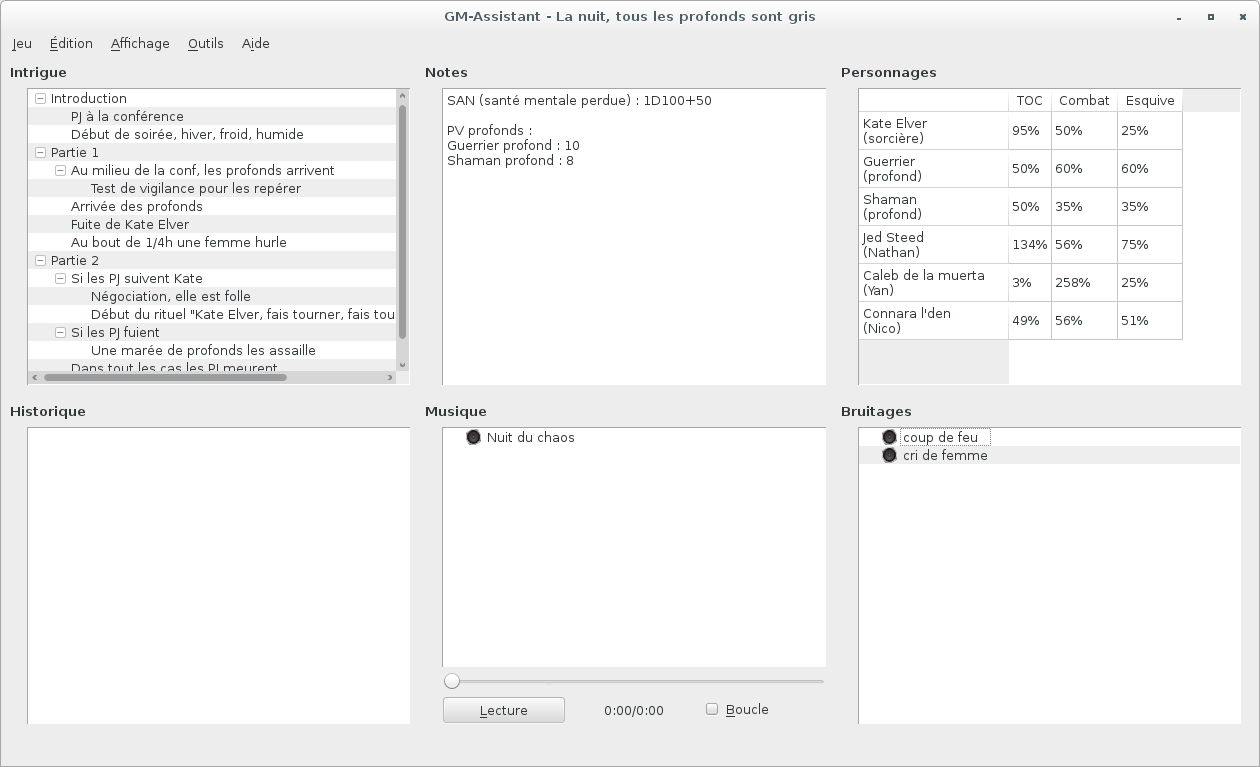
\includegraphics[width=0.9\textwidth]{scenario_complet}
    \caption{La partie est prête}
    \label{scenario_complet}
\end{figure}

Ce fichier scénario est disponible dans le dossier "documentation" de \GMA.

\section{Conclusion}\label{conclusions}
\GMA est un logiciel conçu par des rôlistes pour des rôlistes, c'est-à-dire vous.
Si ce n'est déjà fait, nous vous encourageons à l'essayer.
S'il vous plaît, que vous n'envisagez plus de jouer sans, tant mieux.
Si pour une raison ou une autre ce n'est pas le cas, sachez que nous faisons de notre mieux.
Dans tous les cas, vous êtes cordialement invités à participer à l'amélioration de ce logiciel et ce de plusieurs façons, selon vos compérences et votre motivation~:
\begin{itemize}
    \item en utilisant le logiciel, en nous faisant part de vos impressions, et en signalant d'éventuels bogues~;
    \item en le faisant connaître autour de vous~;
    \item en proposant des fonctionnalités qui pourraient être intégrées à \GMA dans l'avenir~;
    \item en nous aidant à rédiger et relire la documentation~;
    \item en traduisant le logiciel et la documentation dans des langues qui ne sont pas encore supportées~;
    \item en maintenant à jour notre site web \url{http://gmassistant.free.fr}~;
    \item et enfin en rejoignant notre équipe de développeurs.
\end{itemize}

Si vous êtes intéressé, vous pouvez nous joindre à l'adresse \url{gmassistant@free.fr}.
Si vous posséder un compte Github, vous pouvez également suivre l'avancement du projet, jeter un coup d'œil au code et signaler des bogues sur la page du projet \url{http://github.com/ViviCoder/GM-Assistant}.
Enfin, si vous désirez être tenu au courant des dernières actualités concernant GM-Assistant, vous pouvez vous abonner à notre flux RSS (en anglais) \url{http://gmassistant.free.fr/feed}.

\end{document}
